% Kelompok : 5
% Kelas : D4 TI 1A
% Anggota : 
% 1. Harun Ar - Rasyid 	1174027
% 2. Choirul Anam 		1174004
% 3. M.Tomy N.M.		1174031
% 4. Izza				1174013
% 5.Putra				


Artikel ini mengenai segmentation

  \begin{figure}[ht]
  \centerline{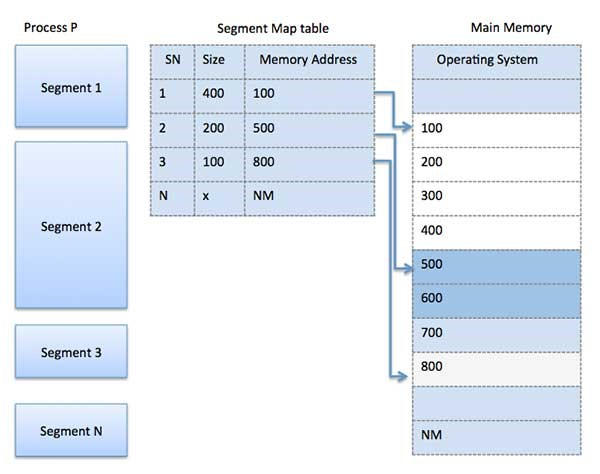
\includegraphics[width=1\textwidth]{..figures/segmentation.jpg}}
  \caption{Contoh segmentation}
  \label{segmentation}
  \end{figure}

\section{Pengertian Segmentation}
ini adalah contoh segmentation \ref{segmentation}
Segmentasi adalah teknik manajemen memori di mana setiap pekerjaan dibagi menjadi beberapa segmen dengan ukuran yang berbeda, satu untuk setiap modul yang berisi potongan-potongan yang melakukan fungsi terkait. Setiap segmen sebenarnya merupakan ruang alamat logis yang berbeda dari program.